
\documentclass{article}

\usepackage[utf8]{inputenc}
\usepackage[left=1.5in,right=1.5in,bottom=1in]{geometry}
 \usepackage{setspace} \onehalfspacing
\setlength\parindent{0pt}
\setlength{\parskip}{1em}
\setcounter{secnumdepth}{0}
\usepackage{outlines}
\usepackage{graphicx}
\usepackage{caption}
\graphicspath{ {imgs} }
\usepackage{hyperref}


\usepackage[
backend=biber,
style=alphabetic,
sorting=ynt
]{biblatex}
\addbibresource{photo_essay.bib}

\title{A walk through Astana's post-modern architecture}
\author{Carla Hyenne}

\begin{document}

\maketitle

\begin{figure}[h!]
	\centering
	\captionsetup{labelformat=empty}
	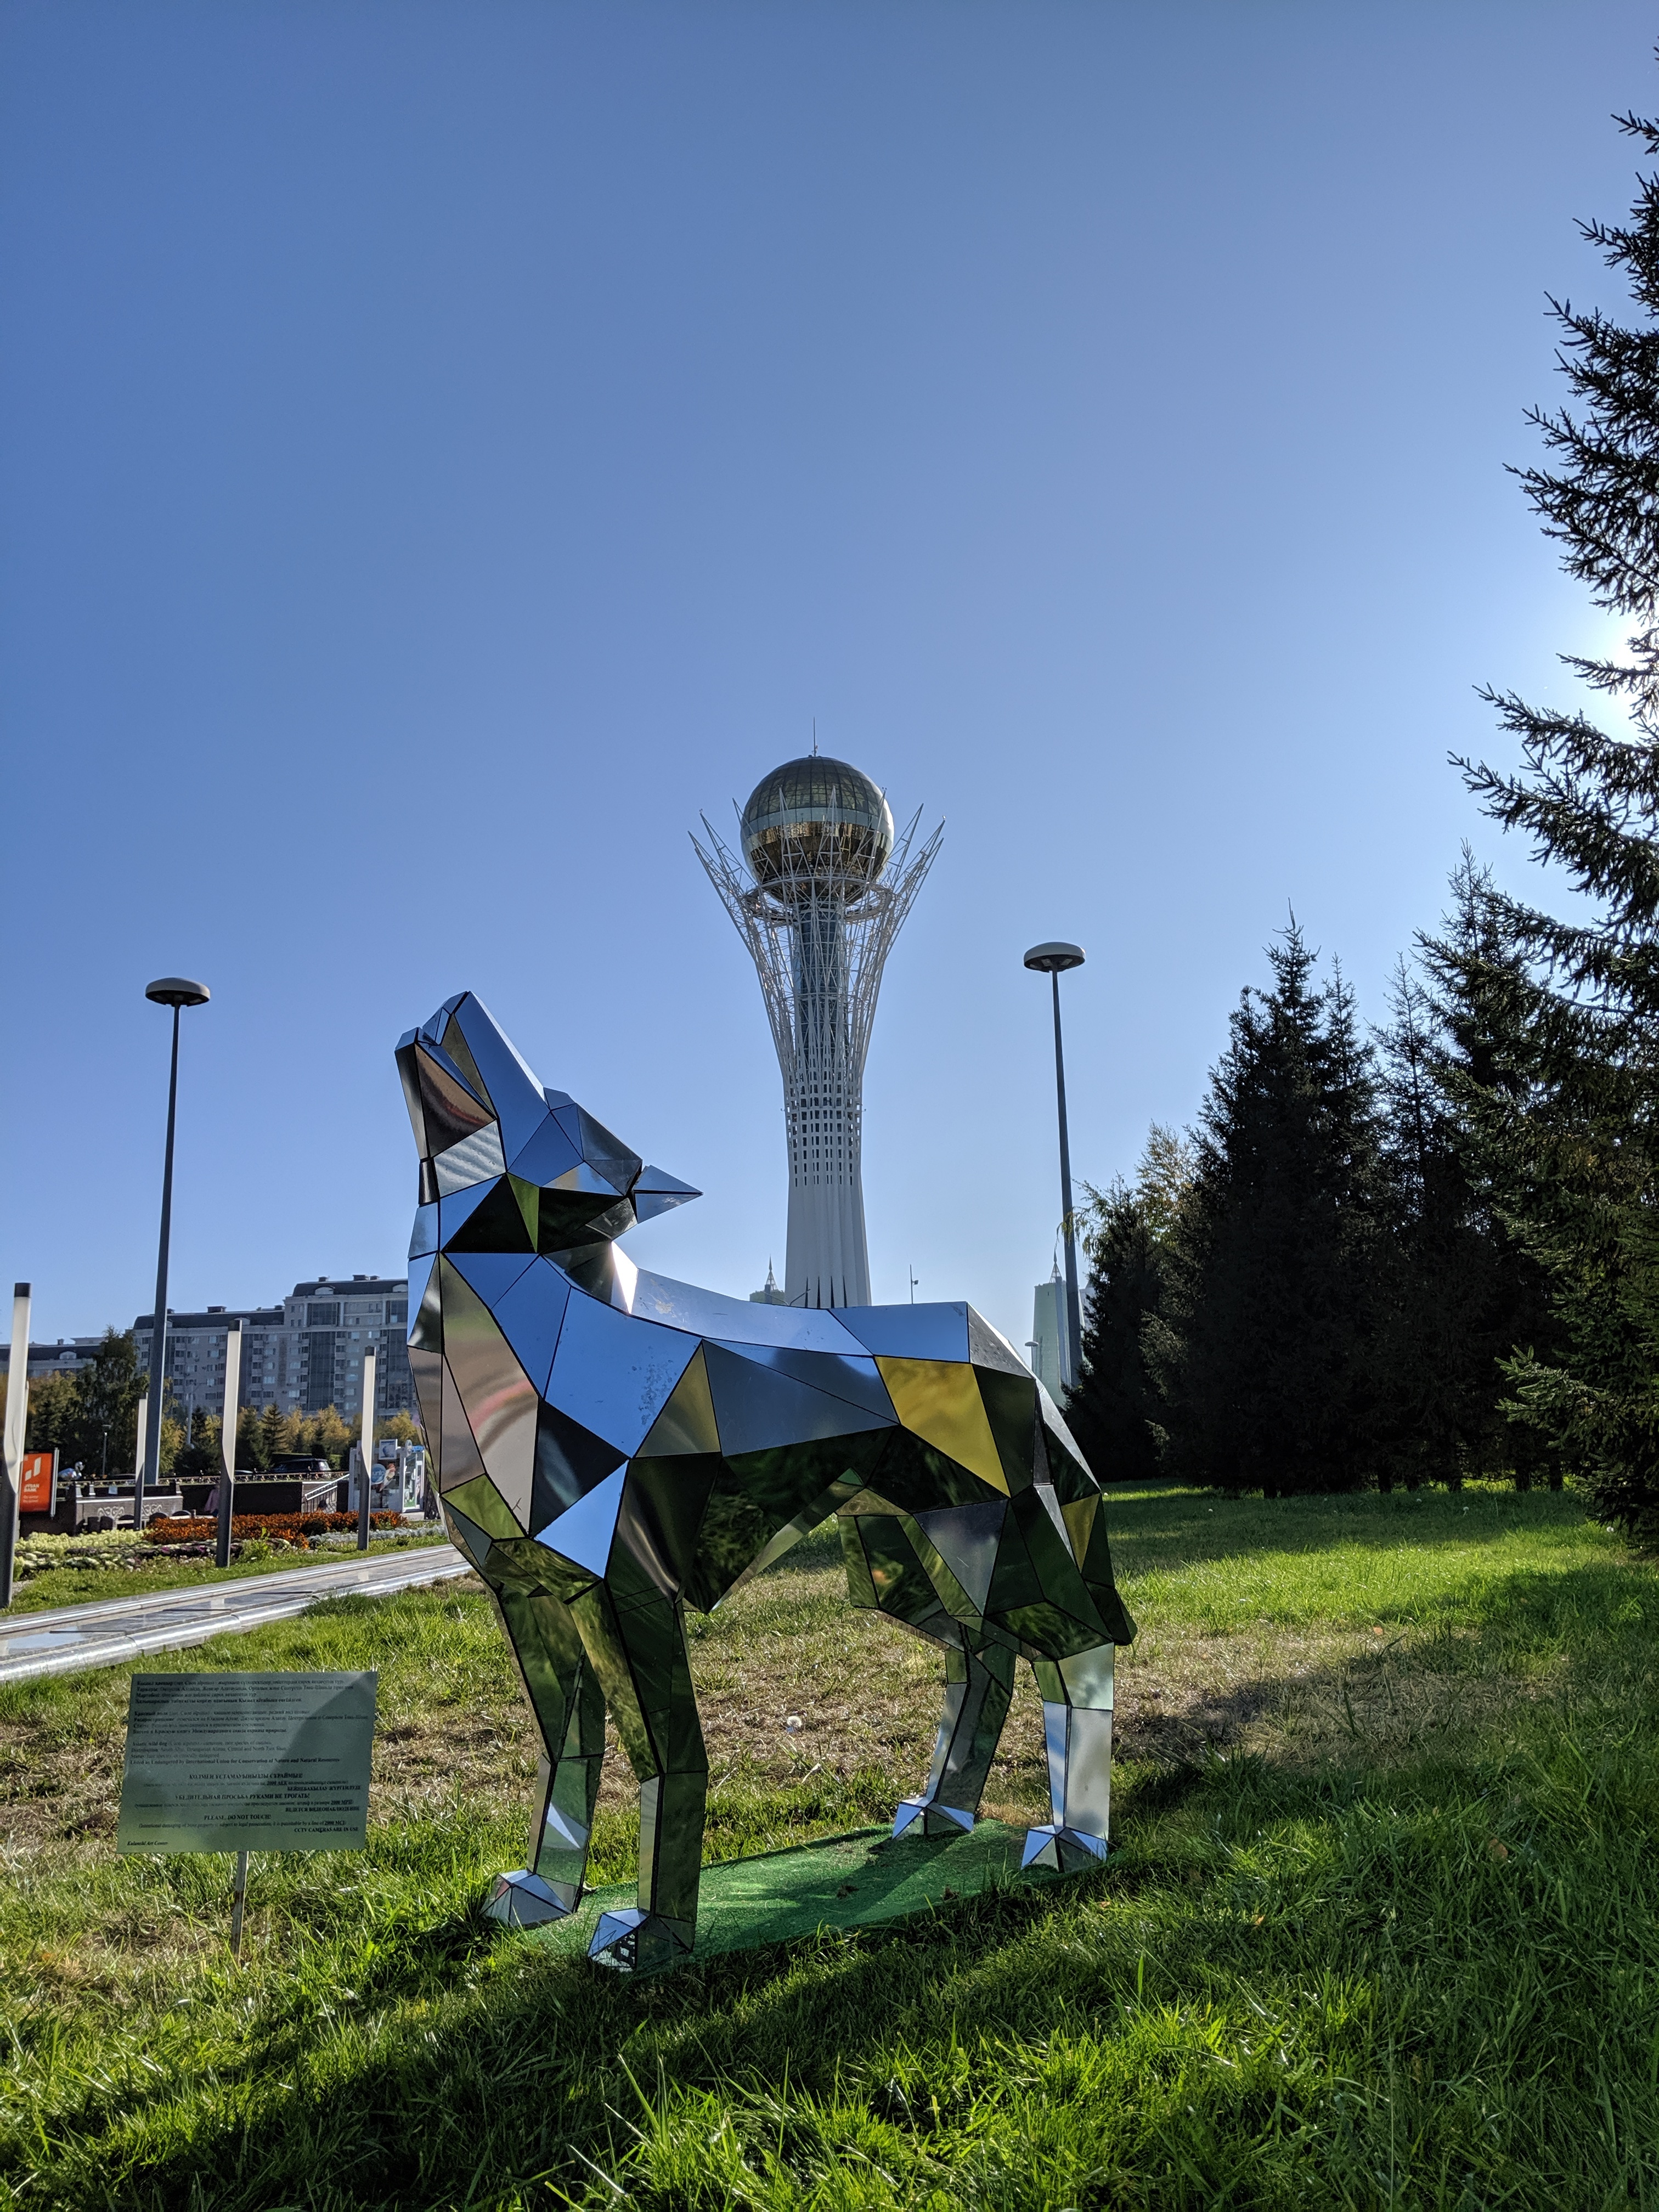
\includegraphics[height=40em]{photo_essay}
	\caption{Astana, October 2019. \textit{Todo image caption}}
\end{figure}

\pagebreak

An ex-soviet state, who's president (Nur Sultan Nazerbayev) was in power for over 20 years, since the country's independence
The capital has an interesting history, moving from Almaty (the biggest city) to Nur Sultan
As a country, KZ is geopolitically complicated: it needs to navigate three of the world's most dominant countries, Russia, China, and the USA. It borders China and Russia, and thus needs to keep close and friendly ties with them. At the same time, not become dependent.
The renaming of Astana to Nur Sultan in 2018 (to be verified) is almost too good to help explain the ideology of the government. President Nazerbayev has an airport, a university, and a city named after him, and the museum of kazakh history (verify) focuses heavily on him as a leader, with a x meter tall statue of him at the centre of a museum.
 The fact that he renamed Astana himself, and that he created his own position as "advisor to the president", also illustrates his authority and, without wanting to draw too many parallels, is reminiscent of Stalin as the "father of the nation" or even Kim Jeong Il as "supreme leader". 
 As a Western woman visiting Kazakhstan and post-soviet, Central Asia for the first time, the propaganda felt so obvious.
 Nonetheless, the people of KZ and especially Astana (I assume, because the rest of the country is not as well off, you can even see it just by crossing the river to the south side of Astana) acknowledge the positive changes that Nazerbayev brought to the city: (verify everything here) better education, infrastructure, modernity...
 
Walking through Astana feels like you have landed in a post-modern, perhaps utopian, city, or even in a science fiction. One massive boulevard (include meters here) cuts through and connects the city. Its lined with impressive building after impressive building. I do not know of another place in the world which has such a display of eclectic, futurist architecture.

Even if we ignore the look of the architecture, the sheer scale of buildings is staggering. On the map, nothing looks particularly far apart. But the length and width of the boulevards are astonishing. The size of the mosque is disorienting, dwarfing. As you can see, it is hard to even get a picture. 
This enormous scale makes it hard to reach any destination without a car or a taxi (insert uber equivalent name here), even if taking a car ride at peak hours might seem slower than walking pace. 
For reference, the presidential palace that is modelled after the white house, is eight times bigger than it. What kind of message is this sending? 

One can't help to wonder, what is behind this architecture? What is the purpose of such a display? Especially as you cross the Isim (?) river towards the south side of Astana, where the modernism stops and low rise, dirty white and brown buildings are the majority. The overwhelming architecture is no where to be seen, and you start to get a sense of neighbourhood and community life. Is this disinvestment? Will creative destruction take over?

Astana is surrounded by steppe, and will not run into space constraints any time soon. 

Did the capital move from Almaty to Astana so that the government could build a city from scratch, and impress the rest of the world? Seem like a big player against Russia and China? Is it meant to intimidate and remind them that KZ is a powerful country who will not let other (communist) countries govern them?  \cite{einstein}


The people of KZ continue to call the city Astana. Even I, as a tourist and someone who has little ties to the country besides a handful of friends, find it odd to call it Nur Sultan. Is this a form of resistance, or a habit that will soon be broken?

\pagebreak

\printbibliography 

\end{document}
